\documentclass[preprint,12pt,a4paper]{elsarticle}
\usepackage{amssymb}
\usepackage{lineno}
\usepackage{float}
\restylefloat{table}
\usepackage[colorlinks=true, urlcolor=blue, pdfborder={0 0 0}]{hyperref}
\usepackage{breakurl}
\usepackage{placeins}
\usepackage{geometry}

\geometry{left=1in, right=1in, top=1in, bottom=1in, headsep=0pt}

\journal{SoftwareX}

\begin{document}
\begin{frontmatter}

\title{Davos: a Python package ``smuggler'' for constructing
  lightweight reproducible notebooks}
\author{Paxton C. Fitzpatrick}
\author{Jeremy R. Manning\corref{cor}}
\ead{Jeremy.R.Manning@Dartmouth.edu}
\cortext[cor]{Corresponding author}
\address{Department of Psychological and Brain Sciences\\Dartmouth College, Hanover, NH 03755}


\begin{abstract}
  Reproducibility is a core requirement of modern scientific research.
  For computational research, reproducibility means that code should
  produce the same results, even when run on different systems.  A
  standard approach to ensuring reproducibility entails packaging a
  project's dependencies along with its primary code base.  Existing
  solutions vary in how deeply these dependencies are specified,
  ranging from virtual environments, to containers, to virtual
  machines.  Each of these existing solutions requires installing or
  setting up a system for running the desired code, increasing the
  complexity and time cost of sharing or engaging with reproducible
  science. Here, we propose a lighter-weight solution: the
  Davos package.  When used in combination with a
  notebook-based Python project, Davos provides a mechanism
  for specifying the correct versions of the project's
  dependencies directly within the code that requires them,
  and automatically installing them in an isolated environment
  when the code is run. The Davos package further
  ensures that these packages and specific versions are used every
  time the notebook's code is executed.  This enables researchers to
  share a complete reproducible copy of their code within a single
  Jupyter notebook file.
\end{abstract}


\begin{keyword}
  Reproducibility \sep Open science \sep Python \sep Jupyter Notebook
  \sep Google Colaboratory \sep Package management
\end{keyword}

\end{frontmatter}


\section*{Metadata}

\section*{Current code version}

\begin{table}[H]
\begin{tabular}{|l|p{6.5cm}|p{6.5cm}|}
\hline
\textbf{Nr.} & \textbf{Code metadata description} & \textbf{Metadata value} \\
\hline
C1 & Current code version &  v0.2.4 \\
\hline
C2 & Permanent link to code/repository used for this code version & \url{https://github.com/ContextLab/davos/tree/v0.2.4} \\
\hline
C3 & Code Ocean compute capsule & \\
\hline
C4 & Legal Code License & MIT \\
\hline
C5 & Code versioning system used & git \\
\hline
C6 & Software code languages, tools, and services used & Python, JavaScript, PyPI/pip, IPython, Jupyter, ipykernel, PyZMQ.\newline Additional tools used for tests: pytest, Selenium, Requests, mypy, GitHub Actions \\
\hline
C7 & Compilation requirements, operating environments, and
     dependencies & Dependencies:~Python $\geq 3.6$, packaging, setuptools.\newline Supported OSes: MacOS, Linux, Unix-like.\newline Supported IPython environments: Jupyter Notebooks, JupyterLab, Google Colaboratory, Binder, IDE-based notebook editors, IPython shell. \\
\hline
C8 & Link to developer documentation/manual & \url{https://github.com/ContextLab/davos\#readme} \\
\hline
C9 & Support email for questions & \href{mailto:contextualdynamics@gmail.com}{contextualdynamics@gmail.com} \\
\hline
\end{tabular}
\caption{Code metadata}
\label{}
\end{table}

\linenumbers


\section{Motivation and significance}

The same computer code may not behave identically under different
circumstances.  For example, when code depends on external packages,
different versions of those packages may function differently.  Or
when CPU or GPU instruction sets differ across machines, the same
high-level code may be compiled into different machine instructions.
Because executing identical code does not guarantee identical
outcomes, code sharing alone is often insufficient for enabling
researchers to reproduce each other's work, or to collaborate on
projects involving data collection or analysis.

Within the Python~\cite{vanR95} community, external packages that are
published in the most popular repositories~\cite{Pyth03, cond15} are
associated with version numbers and tags that allow users to guarantee
they are installing exactly the same code across different computing
environments~\cite{CoghStuf13}.  While it is \textit{possible} to
manually install the intended version of every dependency of a Python
script or package, manually tracking down those dependencies can
impose a substantial burden on the user and create room for mistakes
and inconsistencies. Further, when dependency versions are left
unspecified, replicating the original computing environment becomes
difficult or impossible~\citep{PimeEtal19}.

\begin{figure}[tp]
\centering
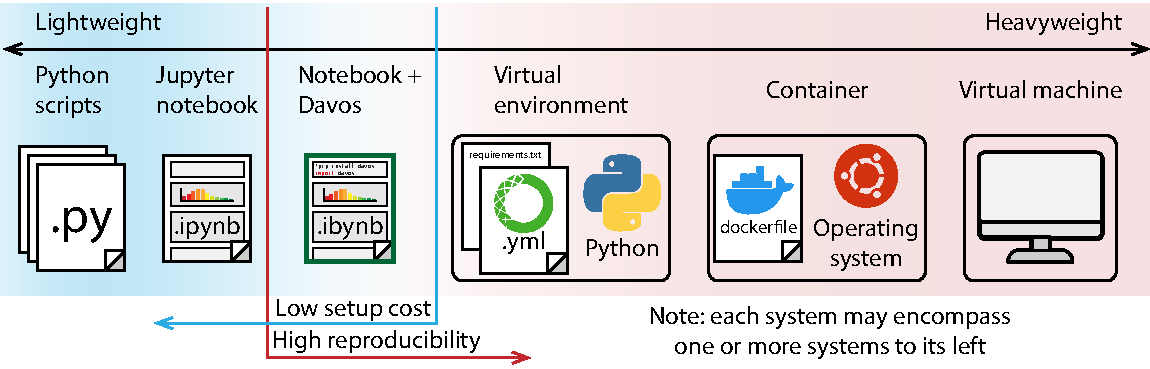
\includegraphics[width=\textwidth]{figs/shareable_code}
\caption{\small \textbf{Systems for sharing code within the Python
  ecosystem.}  From left to right: plain-text \textbf{Python
  scripts} (\texttt{.py} files) provide the most basic ``system''
  for sharing raw code.  Scripts may reference external packages, but
  those packages must be manually installed on other users' systems.
  Further, any checking needed to verify that the correct versions of
  those packages were installed must also be performed manually.
  \textbf{Jupyter notebooks} (\texttt{.ipynb} files) comprise embedded
  text, executable code, and media (including rendered figures, code
  output, etc.).  When the \textbf{Davos package} is imported
  into a Jupyter notebook, the notebook's functionality is extended to
  automatically install any required external packages (at their
  correct versions, when specified).  \textbf{Virtual environments}
  allow users to install an isolated copy of Python and all required
  dependencies. This typically entails distributing a configuration
  file (e.g., a \texttt{pyproject.toml}~\cite{CannEtal16} or
  \texttt{environment.yml} file) that specifies all project
  dependencies (including version numbers of external packages)
  alongside the primary code base. Users can then install a
  third-party tool~\cite[e.g.,][]{Anac12, Eust19} to read the file and
  build the environment.  \textbf{Containers} provide a means of
  defining an isolated environment that includes a complete operating
  system (independent of the user's operating system), in addition to
  (optionally) specifying a virtual environment or other
  configurations needed to provide the necessary computing
  environment.  Containers are typically defined using specification
  files (e.g., a plain-text \texttt{Dockerfile}) that instruct the
  virtualization engine regarding how to build the containerized
  environment.  \textbf{Virtual machines} provide a complete
  hardware-level simulation of the computing environment.  In addition
  to simulating specific hardware, virtual machines (typically
  specified using binary image files) must also define operating
  system-level properties of the computing environment.  Systems to
  the left of the blue vertical line entail sharing individual files,
  with no additional installation or configuration needed to run the
  target code.  Systems to the right of the red vertical line support
  precise control over dependencies and versioning.  Notebooks
  enhanced using the Davos package are easily shareable and
  require minimal setup costs, while also facilitating high
  reproducibility by enabling precise control over project
  dependencies.}
\label{fig:code-sharing}
\end{figure}

Computational researchers and other programmers have de\-vel\-oped a
broad set of approaches and tools to facilitate code sharing and
reproducible outcomes (Fig.~\ref{fig:code-sharing}). At one extreme,
simply distributing a set of Python scripts (\texttt{.py} files) may
enable others to use or gain insights into the relevant work. Because
Python is installed by default on most modern operating systems, for
some projects, this may be sufficient. Another popular approach
entails creating Jupyter notebooks~\cite{KluyEtal16} that comprise a
mix of text, executable code, and embedded media. Notebooks may call
or import external scripts or packages---or even intersperse snippets
of other programming or markup lang\-uages---in order to provide a
more compact and readable experience for users. Both of these systems
(Python scripts and notebooks) provide a convenient means of sharing
code, with the caveat that they do not specify the computing
environment in which the code is executed. Therefore the functionality
of code shared using these systems cannot be guaranteed across
different users or setups.

At another extreme, virtual machines~\cite{Gold74, AltiEtal05, Rose99}
provide a hardware-level simulation of the desired system.  Virtual
machines are typically isolated, such that installing or running
software on a virtual machine does not impact the user's primary
operating system or computing environment.
Containers~\cite[e.g.,][]{Merk14, KurtEtal17} provide a similar
``isolated'' experience. Although containerized environments do not
specify hardware-level operations, they are typically packaged with a
complete operating system, in addition to a complete copy of Python
and any relevant package dependencies. Virtual
environments~\cite[e.g.,][]{Anac12, Eust19} also provide a computing
environment that is largely separated from the user's main
environment. They incorporate a copy of Python and the target
software's dependencies, but virtual environments do not specify or
reproduce an operating system for the runtime environment. Each of
these systems (virtual machines, containers, and virtual environments)
guarantees (to differing degrees---at the hardware level, operating
system level, and Python environment level, respectively) that the
relevant code will run similarly for different users. However, each of
these systems also relies on additional software that can be complex
or resource-intensive to install and use, creating potential barriers
to both contributing to and taking advantage of open science
resources.

We designed Davos to occupy a ``sweet spot'' between these extremes.
Davos is a notebook-installable package that adds functionality to the
default notebook experience. Like standard Jupyter notebooks,
Davos-enhanced notebooks allow researchers to include text, executable
code, and media within a single file. No further setup or installation is
required from the user, beyond what is needed to run standard Jupyter
notebooks. And like virtual environments, Davos provides a convenient
mechanism for fully specifying (and installing, as needed) a complete set of
Python dependencies, including specific package versions, which are contained
and isolated from the rest of the user's system.


\section{Software description}

The Davos package is named after Davos Seaworth, a smuggler referred
to as ``the Onion Knight" from the series \textit{A Song of Ice and Fire} by
George R. R. Martin~\cite{Mart98}. The \texttt{smuggle} keyword provided by
Davos is a play on Python's \texttt{import} keyword: whereas importing
can load a package into the Python workspace within the existing rules and
frameworks provided by the Python language, ``smuggling'' provides an
alternative that expands the scope and reach of ``importing.'' Like the
character Davos Seaworth (who became famous for smuggling onions through a
blockade on his homeland), we use ``onion'' comments to precisely control how
packages are smuggled into the Python workspace.

\begin{figure}[tp]
\centering
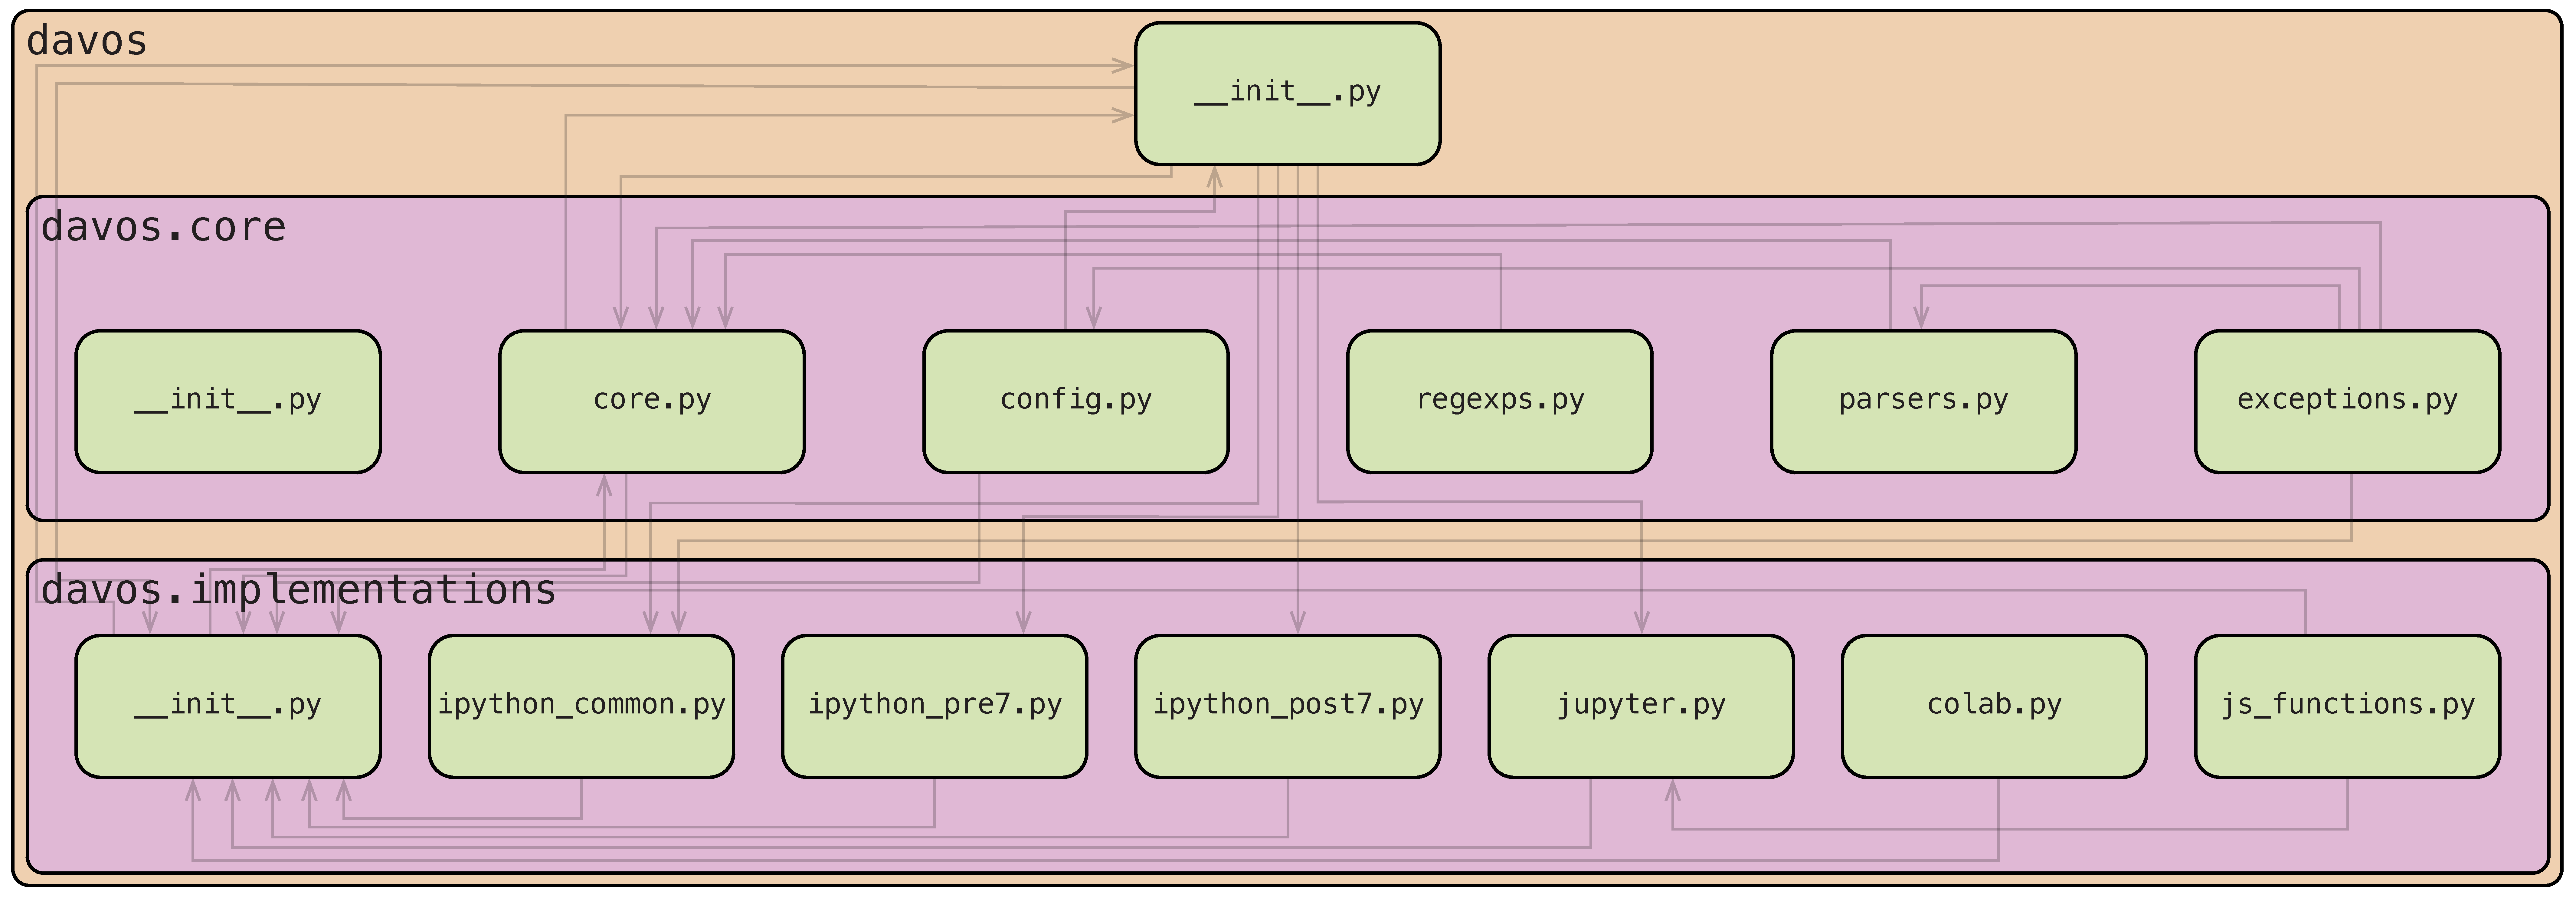
\includegraphics[width=\textwidth]{figs/package_structure}
\caption{\small \textbf{Package structure.} The Davos package
  comprises two interdependent subpackages.  The \texttt{davos.core}
  subpackage includes modules for parsing \texttt{smuggle} statements
  and onion comments, installing and validating packages, isolating and managing
  installed packages, and configuring Davos's behavior.  The
  \texttt{davos.implementations} subpackage includes
  environment-specific modifications and features that are needed to
  support the core functionality across different notebook-based
  environments.  Individual modules (i.e., \texttt{.py} files) are represented by lime
  rounded rectangles, and arrows denote dependencies (each arrow
  points to a module that imports objects defined in the module at the
  arrow's source).}
\label{fig:package-structure}
\end{figure}


\subsection{Software architecture}\label{sec:architecture}

The Davos package consists of two interdependent subpackages
(see Fig.~\ref{fig:package-structure}). The first,
\texttt{davos.core}, comprises a set of modules that
implement the bulk of the package's core
functionality, including pipelines for installing and validating
packages, custom parsers for the \texttt{smuggle} statement (see
Sec.~\ref{subsec:smuggle}) and onion comment (see
Sec.~\ref{subsec:onion}), a system for isolating dependencies of
different projects (see Sec.~\ref{subsec:projects}), and a runtime
interface for configuring Davos's behavior (see Sec.~\ref{subsec:config}).
However, certain critical aspects of this
functionality require (often substantially) different implementations
depending on properties of the notebook environment in which
Davos is used (e.g., whether the frontend is provided by
Jupyter or Google Colaboratory, or which version of
IPython~\cite{PereGran07} is used by the notebook kernel). To deal
with this, environment-dependent components of core features and behaviors
are isolated and abstracted to ``helper functions'' in the
\texttt{davos.implementations} subpackage. This second subpackage
defines multiple, interchangeable versions of each helper function,
organized into modules by the conditions that trigger their use. At
runtime, Davos detects various features in the notebook
environment and selectively imports a single version of each helper
function into the top-level \texttt{davos.implementations} namespace,
allowing \texttt{davos.core} modules to access the proper
implementations for the current notebook environment in a single,
consistent location. An additional benefit of this design is that it
allows both maintainers and users to easily extend Davos to
support new, updated, or custom notebook variants by adding new
\texttt{davos.implementations} modules that define their own versions
of each helper function, modified from existing implementations as
needed.


\subsection{Software functionalities}

\subsubsection{The \texttt{smuggle} statement}\label{subsec:smuggle}

Functionally, importing Davos in an IPython notebook enables
an additional Python keyword: ``\texttt{smuggle}'' (see
Sec.~\ref{subsec:implementation} for details on how this works).
The \texttt{smuggle} keyword can be used as a drop-in
replacement for Python's built-in \texttt{import} keyword to load
packages, modules, and other objects into the notebook's namespace.
However, whereas \texttt{import} will fail if the requested package is
not installed locally, \texttt{smuggle} statements can handle missing
packages on the fly.  If a smuggled package does not exist in the
user's Python environment, Davos will download and install it automatically,
expose its contents to Python's \texttt{import} machinery, and load it
into the notebook for immediate use.

Importantly, packages installed by Davos are made available for use in the
notebook without affecting the user's Python environment or existing packages.
By default, \texttt{smuggle} statements will install missing packages (and any
missing dependencies of those packages) into a notebook-specific, virtual
environment-like directory called a ``project'' (see
Sec.~\ref{subsec:projects}). In turn, \texttt{smuggle} statements executed in a
particular notebook will preferentially load packages from that notebook's
project directory whenever they are available, rather than searching for them
in the user's main Python environment. In this way, \texttt{smuggle}
statements can be substituted for \texttt{import} statements to automatically
ensure that all packages needed to run a notebook are installed and available
at runtime each time the notebook is run, without risking interfering with
dependencies of the user's other Python programs, or other Davos-enhanced
notebooks.


\subsubsection{The onion comment}\label{subsec:onion}

For greater control over the behavior of \texttt{smuggle} statements, Davos
defines an additional construct called the ``onion comment.'' An onion comment
is a special type of inline comment that may be placed on a line containing a
\texttt{smuggle} statement to customize how Davos searches for the smuggled
package locally and, if necessary, downloads and installs it. Onion comments
follow a simple format based on the ``type comment'' syntax introduced in PEP
484~\cite{vanREtal14}, and are designed to make managing packages with Davos
intuitive and familiar. To construct an onion comment, users provide the name
of the installer program (e.g., \texttt{pip}) and the same arguments one would
use to manually install the package as desired via the command line:
\begin{center}
  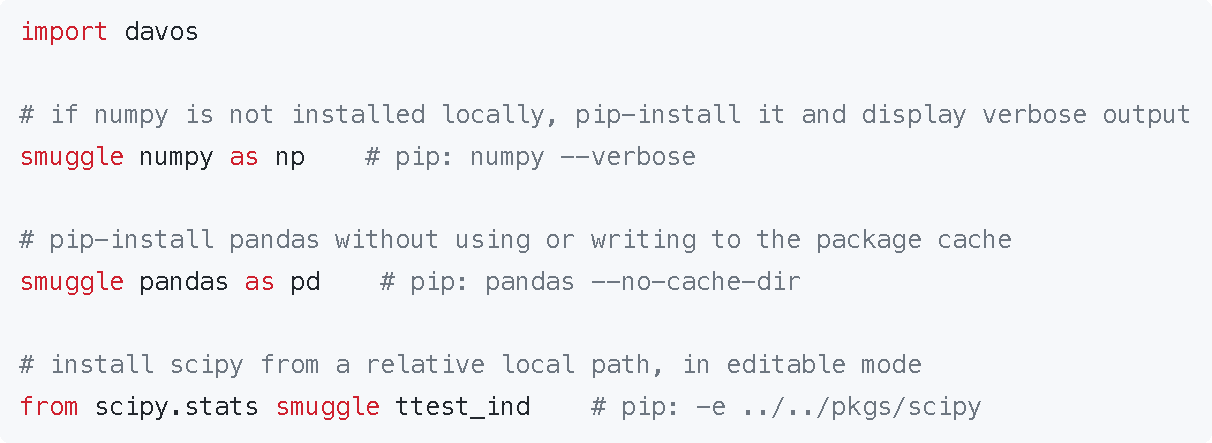
\includegraphics[width=0.9\textwidth]{figs/snippet1}
\end{center}
Occasionally, a package's distribution name (i.e., the name used
when installing it) may differ from its top-level module name (i.e., the name
used when importing it). In such cases, an onion comment can be used to ensure
that Davos installs the proper package if it cannot be found locally:
\begin{center}
  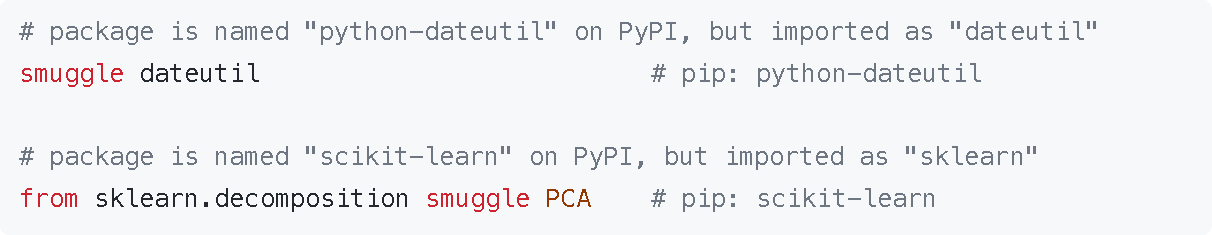
\includegraphics[width=0.9\textwidth]{figs/snippet2}
\end{center}
Because onion comments may be constructed to specify any aspect of
the installer program's behavior, they provide a mechanism for precisely controlling
how, where, and when smuggled packages are installed. Critically, if an onion
comment includes a version specifier~\cite{CoghStuf13}, Davos will ensure that
the version of the package loaded into the notebook matches the specific
version requested (or satisfies the given version constraints). If the smuggled
package exists locally, Davos will extract its version information from its
metadata and compare it to the specifier provided. If the two are incompatible
(or no local installation is found), Davos will download, install, and load a
suitable version of the package instead:
\begin{center}
  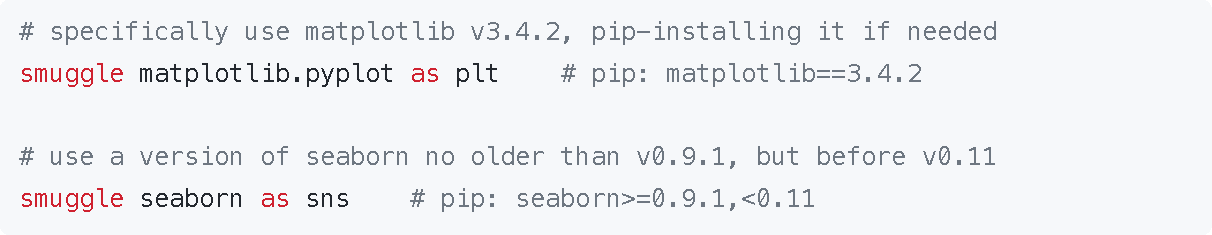
\includegraphics[width=0.9\textwidth]{figs/snippet3}
\end{center}
Onion comments can also be used to \texttt{smuggle} specific VCS references (e.g.,
Git~\cite{TorvHama05} branches, commits, tags, etc.):
\begin{center}
  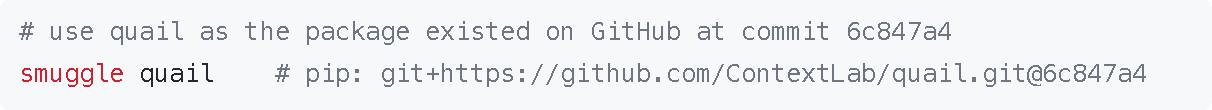
\includegraphics[width=0.9\textwidth]{figs/snippet4}
\end{center}
Davos processes onion comments internally before forwarding arguments to the
installer program. In addition to preventing shared notebooks from executing
arbitrary code in a user's shell, this enables Davos to adjust its behavior
based on how particular flags will affect the behavior of the installer
program. For example, including \texttt{pip}'s \texttt{--no-input} flag will also
temporarily enable Davos's non-interactive mode (see Sec.~\ref{subsec:config}).
Similarly, if an onion comment contains either \texttt{-I}/\texttt{--ignore-installed},
\texttt{-U}/\texttt{--upgrade}, or \texttt{--force-reinstall}, Davos will
install and load a new copy of the smuggled package without first checking
for it locally:
\begin{center}
  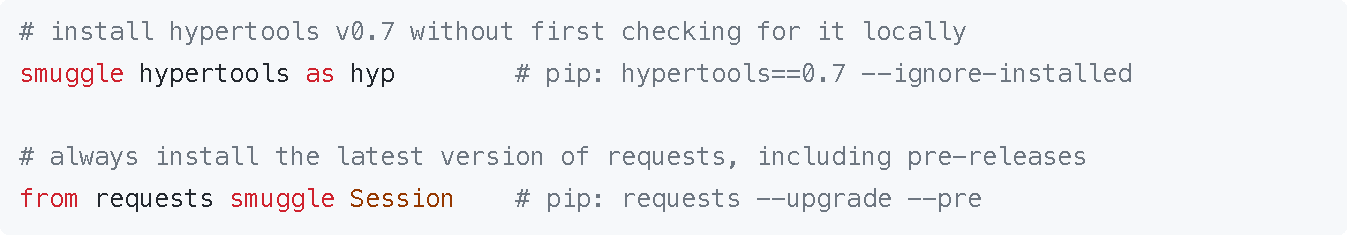
\includegraphics[width=0.9\textwidth]{figs/snippet5}
\end{center}
Since the purpose of an onion comment is to describe how a smuggled package
should be installed (if necessary) so that it can be loaded and used
immediately, options that would normally cause the package not to be installed
(such as \texttt{-h}/\texttt{--help} or \texttt{--dry-run}) are disallowed. Additionally,
when using a Davos ``project'' to isolate smuggled packages (the default behavior;
see Sec.~\ref{subsec:projects}), onion comments may not contain options that
would change the package's installation location (such as
\texttt{-t}/\texttt{--target}, \texttt{--root}, or \texttt{--prefix}). However, if
the user disables project-based isolation and specifies \texttt{--target <dir>},
Davos will ensure that \texttt{<dir>} is included in the module search path (i.e.,
\texttt{sys.path}), prepending it if necessary, so the package can be loaded.


\subsubsection{Projects}\label{subsec:projects}

Standard approaches to installing packages from within a notebook can alter the local Python environment in potentially unexpected and undesired ways.
For example, running a notebook that installs its dependencies via system shell commands (prefixed with ``\texttt{!}'') or IPython magic commands (prefixed with ``\texttt{\%}'') may cause other existing packages in the user's environment to be uninstalled and replaced with alternate versions.
This can lead to incompatibilities between installed packages, affect the behavior of the user's other scripts or notebooks, or even interfere with system applications.

To prevent Davos-enhanced notebooks from having unwanted side effects on the user's environment, any packages installed via \texttt{smuggle} statements are automatically isolated using a custom, virtual environment-like system called ``projects.''
Davos projects are similar to standard Python virtual environments (e.g., created with the standard library's \texttt{venv} module or a third-party tool like \texttt{virtualenv}~\cite{BickEtal07}) but with a few noteworthy differences that make them generally lighter-weight and simpler to use.
Like a standard virtual environment, a Davos project consists of a directory (within a hidden \texttt{.davos} folder in the user's home directory) that houses third-party packages needed for a particular Python project, workflow, or task.
However, unlike standard virtual environments, Davos projects do not need to be manually created, activated, or deactivated,
%and work by \textit{supplementing} the user's existing Python environment rather than replacing it.
and function to \textit{extend} the user's existing Python environment rather than replace it.

When Davos is imported into a notebook, a project directory for that notebook is automatically created (if it does not exist already).
When \texttt{smuggle} statements within that notebook are then executed, any packages (or specific versions of packages) that are not already available in the user's Python environment are installed into the notebook's project directory (along with any missing dependencies of those packages).
During each \texttt{smuggle} statement's execution, Davos also temporarily prepends the notebook's project directory to the module search path so that these project-installed packages are visible when searching for smuggled packages locally, and prioritized over those in the user's main environment.

Thus, rather than constructing fully separate Python environments from scratch,
%Davos projects serve to fill in the gap between the user's existing environment and the dependencies of their corresponding notebooks.
Davos projects work by supplementing the user's existing environment with any additional packages (or specific package versions) needed to satisfy the dependencies of their corresponding notebooks.
In some cases, this might include every package smuggled into a notebook (e.g., if the notebook is run inside a freshly created, empty virtual environment).
In other cases, the user's environment may already provide all required packages, and the notebook's project directory will go unused (in which case it will be deleted automatically when the notebook kernel is shut down).
But regardless of the extent to which the existing environment is augmented, Davos's project system ensures that all smuggled packages are installed locally and loaded successfully at runtime, while the contents of the user's Python environment are never altered.

Additionally, because \texttt{smuggle} statements in a given notebook are evaluated every time it is run, this system also ensures that the notebook's requirements will remain satisfied even if the user's Python environment changes.
For example, suppose a user has \texttt{NumPy}~\cite{HarrEtal20} v1.24.3 installed in their current Python environment and runs a Davos-enhanced notebook that smuggles \texttt{NumPy} with ``\texttt{numpy==1.24.3}'' specified in an onion comment (see Sec.~\ref{subsec:onion}).
Since the user's existing version of the package satisfies this requirement, Davos will happily load it into the notebook.
But if the user later upgrades their environment's \texttt{NumPy} version to v1.25.0 (perhaps as a result of installing a different package that depends on it) and subsequently reruns this notebook, the local version will longer satisfy this requirement, so Davos will install \texttt{NumPy} v1.24.3 into the notebook's project directory and load that version instead.
From then on, any further changes to the user's \texttt{Numpy} installation would have no effect on Davos's behavior in this particular notebook, as a satisfactory version now exists in its project directory.
(If the version specified in the onion comment were changed, Davos would update the version installed in the project directory accordingly.)
For efficiency, Davos projects will generally not duplicate dependencies already satisfied by the user's Python environment.
However, if desired, adding \texttt{pip}'s \texttt{--ignore-installed} flag to an onion comment in the notebook will cause Davos to install the smuggled package into the project directory whether or not it already exists locally.

By default, each Davos-enhanced notebook will create and use its own notebook-specific project named for the absolute path to the notebook file.
However, before smuggling its required packages, a notebook may be set to instead use an arbitrarily named, notebook-agnostic project by assigning any (non-empty) string to \texttt{davos.project} (see Sec.~\ref{subsec:config}).
This provides a convenient way for multiple related notebooks that share a common set of requirements to use the same Davos project, by setting \texttt{davos.project} to the same string in each one.
%This provides a convenient way to share a single Davos project across multiple related notebooks that share a common set of requirements, by setting \texttt{davos.project} to the same string in each one.
It is also possible (though not recommended) to disable Davos's project system entirely and install smuggled packages directly into the user's Python environment by setting \texttt{davos.project} to \texttt{None}.

When accessed (unless its value has been set to \texttt{None}), \texttt{davos.project} will return a \texttt{Project} object that represents the project used by the current notebook (strings assigned to \texttt{davos.project} are converted to \texttt{Project}s internally). This object supports methods for interacting with the current project, including locating its directory on the file system, listing all installed packages' names and versions, changing the project's name, and deleting its contents altogether.
\texttt{Project} instances can also be created and managed programmatically, and Davos provides additional utilities for viewing and working with all existing projects (see Secs.~\ref{subsec:config} and \ref{subsec:toplevel}).
\textcolor{red}{\textbf{TODO}: mention \texttt{AbstractProject}s? Note default project name if imported in IPython shell, or fail to get notebook name?}



\subsubsection{Configuring and querying Davos}\label{subsec:config}

After importing Davos into a notebook, the top-level \texttt{davos} module exposes a set of attributes whose values determine various aspects of Davos's behavior. Most of these attributes are writeable options that can be modified to customize how, where, and when Davos installs smuggled packages (see Sec.~\ref{sec:illustrative-example} for an illustrative example). These include:

%After importing Davos into a notebook, the top-level \texttt{davos} module provides a set of attributes whose values may be displayed interactively, checked programmatically at runtime, or modified to customize various aspects of Davos's behavior (see Sec.~\ref{sec:illustrative-example} for an illustrative example and Sec.~\ref{subsec:implementation} for implementation details and additional information).
%These writeable attributes include:

%Davos's behavior may be customized by modifying a set of attributes attached to
%the \texttt{davos} module object that is added to the workspace when Davos is
%imported. These attributes may be modified, displayed, or checked
%programmatically at runtime (see Sec.~\ref{sec:illustrative-example} for an
%illustrative example or Sec.~\ref{subsec:implementation} for implementation
%details and additional information). These include:

\begin{itemize}
\item \texttt{.active}: This attribute controls whether support for \texttt{smuggle}
  statements and onion comments is enabled (\texttt{True}) or
  disabled (\texttt{False}).  When Davos is first imported,
  \texttt{davos.active} is set to \texttt{True} (see Sec.~\ref{subsec:implementation} for implementation details and additional information).

\item \texttt{.auto\_rerun}: This attribute controls how
  Davos behaves when attempting to \texttt{smuggle} a new
  version of a package that was previously loaded (via an \texttt{import} or \texttt{smuggle} statement) and cannot be
  reloaded. This can happen if the package includes extension modules
  that dynamically link C or C++ objects to the Python interpreter,
  and the code that generates those objects was changed between the
  previously loaded and to-be-smuggled versions.  If this attribute
  is set to \texttt{True}, Davos will automatically restart
  the notebook kernel and rerun all code up to (and including) the
  current \texttt{smuggle} statement. If set to \texttt{False} (the default),
  Davos will instead issue a warning, pause execution, and
  prompt the user to either restart and rerun the notebook, or
  continue running with the previously loaded package version until
  the next time the kernel is restarted manually.  Note that, as of
  this writing, setting \texttt{davos.auto\_rerun} to \texttt{True} is not
  supported in Google Colaboratory notebooks.

\item \texttt{.confirm\_install}: If set to \texttt{True} (default:
  \texttt{False}), Davos will require user confirmation
  before installing a smuggled package that is not already
  available locally. This is primarily useful if the user has disabled
  Davos's ``project'' system for isolating smuggled packages (see
  Sec.~\ref{subsec:projects}) but still wants to carefully control what
  packages are installed into their main Python environment.

\item \texttt{.noninteractive}: Setting this attribute to
  \texttt{True} (default: \texttt{False}) enables non-in\-ter\-act\-ive
  mode, in which all user interactions (prompts and dialogues) are
  disabled. Note that in non-interactive mode, the
  \texttt{confirm\_install} option is set to \texttt{False}.  If
  \texttt{auto\_rerun} is set to \texttt{False} while in non-interactive
  mode, Davos will raise an exception if a smuggled package
  cannot be reloaded, rather than prompting the user.

\item \texttt{.pip\_executable}: This attribute's value specifies the
  path to the \texttt{pip} executable used to install smuggled
  packages. The default is programmatically determined from the user's Python
  environment and falls back to \texttt{<sys.executable> -m pip} if no
  executable can be found.

\item \texttt{.project}: This attribute's value is a \texttt{Project} instance representing the Davos project associated with the current notebook. As described in Section~\ref{subsec:projects}, Davos projects serve to isolate packages installed by \texttt{smuggle} statements from the user's main Python environment, and the \texttt{Project} class provides an interface for inspecting and managing projects at runtime. This attribute's default value is a notebook-specific project named for the absolute path to the notebook file. To change the project used in the current notebook (e.g., in order to use the same project in multiple related notebooks), this attribute may be assigned a different \texttt{Project} instance or, for simplicity, the name of the desired project as a string or \texttt{pathlib.Path} (either of which will be converted to a \texttt{Project} on assignment). Alternatively, setting \texttt{davos.project} to \texttt{None} will disable project-based isolation for the current notebook and cause Davos to install any missing packages directly into the main Python environment. This attribute can be reset to its default value using the top-level \texttt{use\_default\_project()} function (see Sec.~\ref{subsec:toplevel}). For more information about Davos projects, see Section \ref{subsec:projects}.

\item \texttt{.suppress\_stdout}: If this attribute is set to
  \texttt{True} (default: \texttt{False}), Davos suppresses
  printed (console) outputs from both itself and the installer program.
  This can be useful when smuggling packages that require installing many
  dependencies and/or generate extensive output when built from source distributions. Note that if this option is enabled and the installer
  program throws an error, both its stdout and stderr streams will still be
  displayed alongside the Python traceback to allow for debugging.

\end{itemize}

\noindent The attributes above can be modified directly or via the \texttt{davos.configure()} function, which allows setting multiple options simultaneously (see Sec.~\ref{subsec:toplevel} for more information or Sec.~\ref{sec:illustrative-example} for example usage). In addition to these writeable options, the top-level \texttt{davos} module also exposes several read-only attributes that can be displayed in the notebook or checked programmatically at runtime, and provide potentially useful information about the notebook environment or Davos's internal state:

%\noindent Davos also provides a top-level \texttt{configure()} function that allows setting multiple of the above options simultaneously (see Sec.~\ref{subsec:toplevel} or Sec.~\ref{sec:illustrative-example} for example usage). In addition to these writeable options,
%
% for setting multiple of the above options simultaneously (see Sec.~\ref{sec:illustrative-example} for
%
%\noindent Davos namespace also defines the \texttt{davos.configure()} function,
%which allows setting multiple configuration options simultaneously. In addition
%to the above configurable attributes, the \texttt{davos} object also includes
%several read-only attributes that contain potentially useful information about
%the current environment or Davos's behavior:

\begin{itemize}

\item \texttt{.all\_projects}: This attribute contains a list of all Davos projects that exist on the user's local system (see Sec.~\ref{subsec:projects} for more information about Davos projects). Each item in this list is either a \texttt{Project} or \texttt{AbstractProject} instance. \texttt{AbstractProject}s represent notebook-specific projects whose associated notebooks no longer exist. They support all the same functionality as \texttt{Project} objects (including methods for inspecting, renaming, and deleting them) and serve primarily to help users identify and clean up extraneous projects left behind after deleting Davos-enhanced notebooks (e.g., see Sec.~\ref{subsec:toplevel}).
\textcolor{red}{\textbf{TODO}: mention that project can become AbstractProject when notebook is moved/renamed, and can be re-linked by renaming project to new path?}

\item \texttt{.environment}: This attribute's value is a string denoting the set of environment-dependent ``helper functions'' used by Davos in the current notebook. As described in Section \ref{sec:architecture}, Davos internally chooses between interchangeable implementations of certain core features
%(defined in the \texttt{davos.implementations} subpackage)
based on various properties of the notebook's frontend and IPython kernel. As of this writing, three unique combinations of helper functions are required to support existing notebook environments, ergo this attribute has three possible values: \texttt{"IPython<7.0"}, \texttt{"IPython>=7.0"}, or \texttt{"Colaboratory"}. However, this attribute could take on additional values in the future, as new notebook interfaces are created and IPython's internals are updated, and additional versions of helper functions are added to Davos to support them.

%\item \texttt{.environment}: This attribute's value is a string describing the notebook environment into which Davos was imported. Davos uses this value internally to select between interchangeable implementations of certain core features based on various properties of the current notebook's frontend and IPython kernel (see Sec.~\ref{sec:architecture} and Fig.~\ref{fig:package-structure}). As of this writing, possible values of this attribute are \texttt{"IPython<7.0"}, \texttt{"IPython>=7.0"}, and \texttt{"Colaboratory"}, though additional alternatives may be added in the future as new notebook interfaces and IPython versions are released, and Davos is updated to support them.
 %are released and the IPython ecosystem continues to evolve. \textcolor{red}{\textbf{TODO}: tweak wording to convey new possibilities will be added when new things are released that aren't covered by existing implementations, and davos adds new mutually exclusive ones to support them}

\item \texttt{.ipython\_shell}: This attribute contains the global IPython \texttt{InteractiveShell} instance underlying the notebook kernel session.

\item \texttt{.smuggled}: This attribute's value is a Python dictionary that functions as a cache of \texttt{smuggle} statements executed during the current notebook kernel session. The dictionary's keys are names of smuggled packages, and its values are arguments passed to the installer program via onion comments. Entries appear in order of the \texttt{smuggle} statements' execution.

\end{itemize}

\bigskip\bigskip\textcolor{red}{\textbf{========== TODO: finish editing from here to end ==========}}\bigskip\bigskip

\subsubsection{Other top-level Davos functions}\label{subsec:toplevel}
\textcolor{red}{\textbf{TODO: add content}}
%- .configure()
%- .get_project()
%- .prune_projects()
%- .require_pip()
%- .require_python()
%- .use_default_project()

\subsection{Implementation details}\label{subsec:implementation}

Although Davos is designed to \textit{appear} to add a new
keyword to Python's vocabulary, this illusion is actually created through
several ``hacks'' that make use of the notebook's IPython backend
for processing and executing users' code.  Specifically, when
Davos is first imported, or when it is activated after having been
set to an inactive state, two actions are triggered.  First, the
\texttt{smuggle()} function is injected into the IPython user
namespace.  Second, the Davos parser is registered as a
custom IPython input transformer.

IPython preprocesses all executed code as plain text before it is sent
to the Python compiler, in order to handle special constructs like
\texttt{!}-prefixed shell commands and \texttt{\%}-prefixed ``magic'' commands. Davos uses
%``magic'' (i.e., \texttt{\%}-prefixed) and and `` \texttt{!shell} commands. Davos uses
this process to transform \texttt{smuggle} statements into
syntactically valid Python code. The Davos parser uses a
regular expression to match lines of code containing \texttt{smuggle}
statements (and, optionally, onion comments), extract relevant
information from their text, and replace them with equivalent calls to
the \texttt{smuggle()} function. For example, if a user runs a
notebook cell containing
\begin{center}

\includegraphics[width=0.9\textwidth]{figs/snippet6}
\end{center}
the code that is actually executed by the Python interpreter would be
\begin{center}
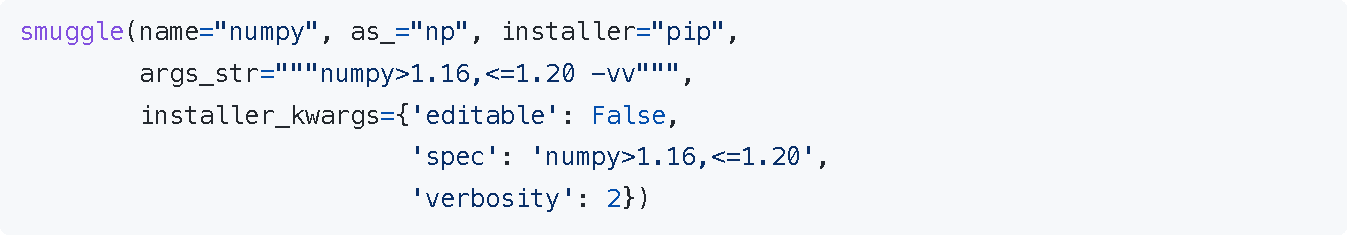
\includegraphics[width=0.9\textwidth]{figs/snippet7}
\end{center}
The call to the \texttt{smuggle()} function carries out
Davos's central logic by determining whether the smuggled
package must be installed, carrying out the installation if necessary,
and subsequently loading it into the namespace. This process is
outlined in Figure~\ref{fig:flow-chart}. Because the
\texttt{smuggle()} function is defined in the notebook namespace, it
is also possible (though never necessary) to call it
directly. Deactivating Davos will delete the name
``\texttt{smuggle}'' from the namespace, unless its value has been
overwritten and no longer refers to the \texttt{smuggle()}
function. It will also deregister the Davos parser from the
set of input transformers run when each notebook cell is
executed. While the overhead added by the Davos parser is
minimal, this may be useful, for example, when optimizing or precisely
profiling code.

\begin{figure}[tp]
\centering
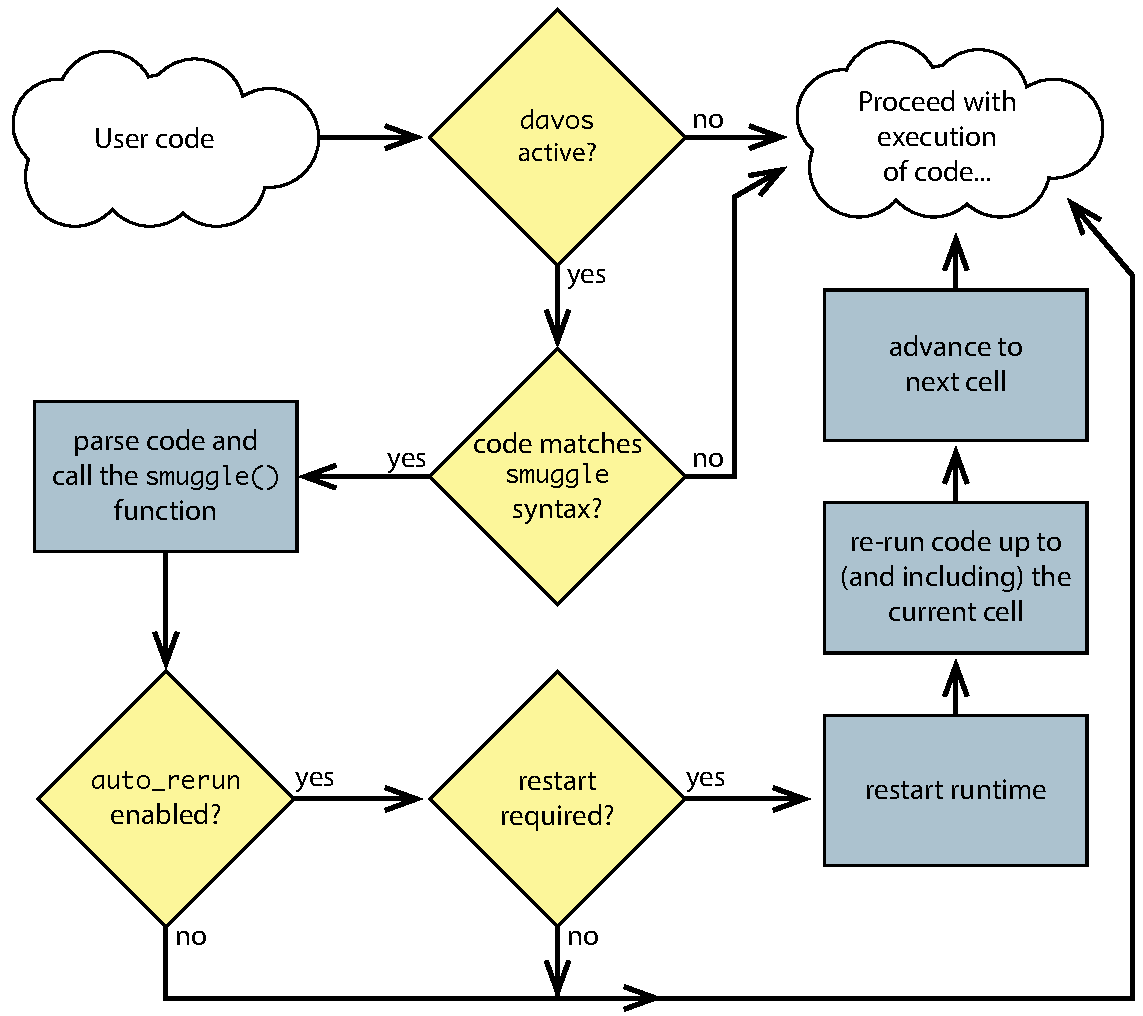
\includegraphics[width=\textwidth]{figs/flow_chart}
\caption{\small \textbf{\texttt{smuggle()} function algorithm.}  At a
  high level, the \texttt{smuggle()} function may be conceptualized as
following two basic steps.  First (left), Davos ensures that the
correct version of the desired package has been installed, carrying
out the installation automatically if needed.  Second (right),
Davos imports the package and updates the current runtime environment.}
\label{fig:flow-chart}
\end{figure}


\section{Illustrative Example}\label{sec:illustrative-example}

\begin{figure}[tp]
\centering
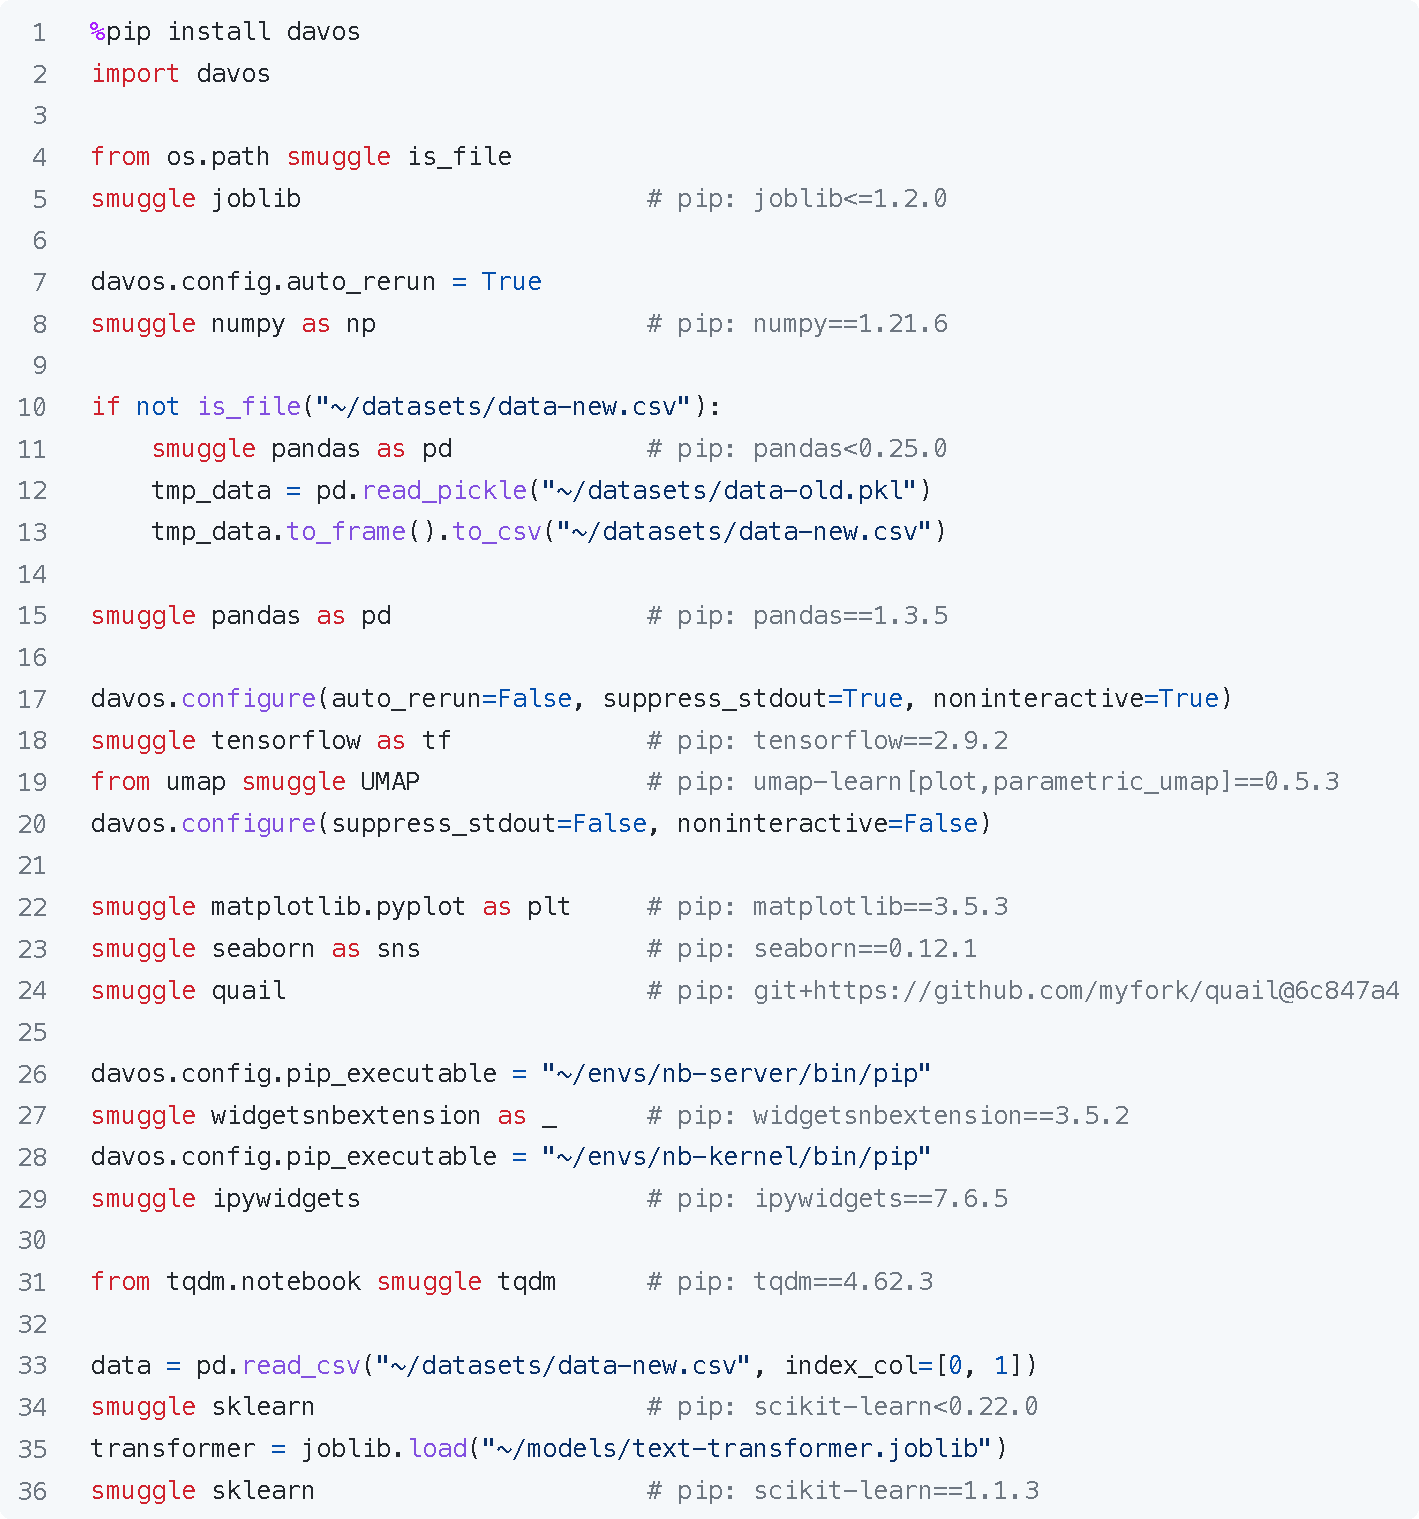
\includegraphics[width=\textwidth]{figs/illustrative_example}
\caption{\small \textbf{Example use case for Davos.}
  Snippets from this example are also excerpted in the main text of
  Section~\ref{sec:illustrative-example}.}
\label{fig:illustrative-example}
\end{figure}

Across different versions of a given package, particular modules, functions,
and other objects may be updated, removed, renamed, or otherwise altered. In
addition to changing the behaviors of active computations, these changes can
render saved objects created using one version of a package incompatible with
other versions of the same package. For example, the popular
\texttt{pandas}~\cite{McKi10} library used to include the \texttt{Panel} data
structure for storing 3-dimensional arrays. Since version 0.20.0, however, the
\texttt{Panel} class has been deprecated, and in version 0.25.0, it was removed
entirely. Suppose a user had a dataset stored in a \texttt{Panel} object
(created using an older version of \texttt{pandas}) and had saved it to their
disk (e.g., for later reuse or to share with other users) by serializing the
\texttt{Panel} with Python's \texttt{pickle} protocol. The \texttt{pickle}
protocol is a popular built-in method of persisting data in Python that allows
users to save, share, and load arbitrary objects. However, in order to
successfully ``unpickle'' (i.e., load and restore) a ``pickled'' (i.e., previously saved)
object, the object's class must be defined in and importable from the same
module as when it was saved. Thus, because of the \texttt{Panel} class's
removal, the user's dataset could not be read by any version of \texttt{pandas}
from 0.25.0 or beyond. These incompatibilities are also not limited solely to
traditional forms of data. For example, saved model states and other objects
may reference modules, functions, attributes, classes, or other objects that
may not be identical (or even present) across all versions of their associated
package.

The example provided in Figure~\ref{fig:illustrative-example} demonstrates how
the Davos package can be used to circumvent these incompatibilities by
carefully controlling which versions of each package are used in different
parts of the notebook. The example shows how a dataset and model that require
now-incompatible components of the \texttt{pandas} and
\texttt{scikit-learn}~\cite{PedrEtal11} packages may be loaded in (using older
versions of each package) and used alongside more recent versions of each
package that provide new and improved functionality. When included at the top
of a Jupyter notebook, the code in Figure~\ref{fig:illustrative-example}
ensures that these objects will be loaded successfully and analyzed using the
same set of package versions, no matter when or by whom the notebook is run.

After installing and importing Davos (lines 1--2), we first \texttt{smuggle} two
utilities for interacting with local files in the code below. The
\texttt{smuggle} statement in line 4 loads the \texttt{is\_file()}
function from the Python standard library's \texttt{os.path}
module. Standard library modules are included with all Python
distributions, so this line is functionally equivalent to an
\texttt{import} statement and does not need or benefit from an onion
comment. Line 5 loads the \texttt{joblib} package~\cite{Varo10},
installing it first, if necessary. Since \texttt{joblib}'s I/O
interface has historically remained stable and backwards-compatible
across releases, requiring that users have a particular exact version
installed would likely be unnecessarily restrictive. However, a
\textit{future} release might introduce some breaking change.  The
onion comment in line 5 helps ensure the analysis notebook continues
to run properly in the future by limiting allowable versions to those
already released when the code was written:
\begin{center}
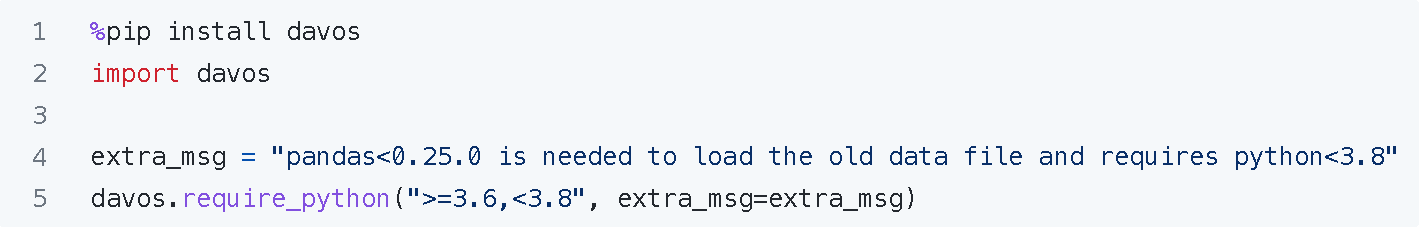
\includegraphics[width=0.9\textwidth]{figs/example1}
\end{center}
Line 7 then uses the \texttt{davos.config} object to enable
Davos's \texttt{auto\_rerun} option before smuggling the next
two packages: \texttt{NumPy} and
\texttt{pandas}. Because these packages rely heavily on custom C data
types, loading the particular versions from the onion comments may
require restarting the notebook kernel if different versions had been previously
imported during the same interpreter session (see
Sec.~\ref{subsec:config}).
\begin{center}
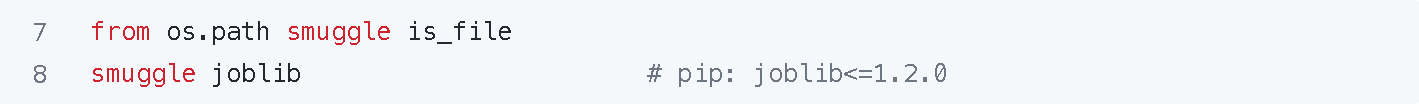
\includegraphics[width=0.9\textwidth]{figs/example2}
\end{center}
Setting the \texttt{auto\_rerun} attribute to \texttt{True} is particularly useful
for managing the installation of \texttt{pandas} in the next
lines:
\begin{center}
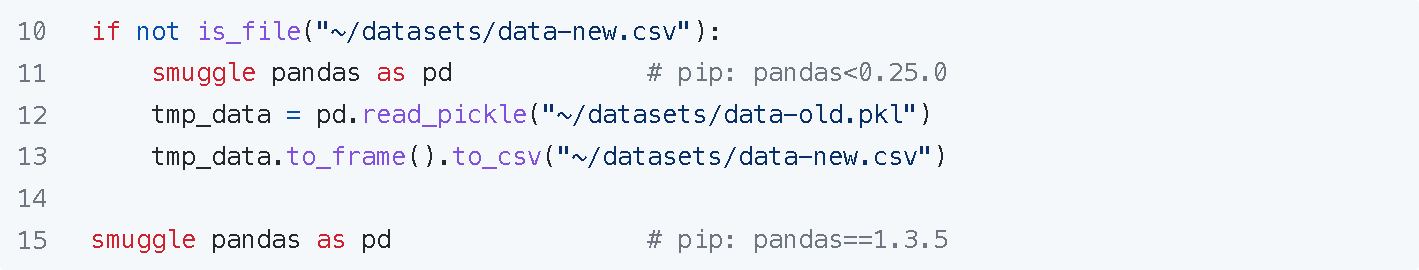
\includegraphics[width=0.9\textwidth]{figs/example3}
\end{center}
If we suppose that the data contained in \texttt{data-old.pkl} is
stored in a pickled \texttt{Panel} object, then we must use a version of
\texttt{pandas} prior to 0.25.0 (i.e., the version in which the \texttt{Panel}
class was removed) to be able to load it in. Line 11 ensures
that an older version of \texttt{pandas} will be imported, enabling
the data to be read in (and, in line 13, written to a CSV
file, which is compatible with newer \texttt{pandas} versions).

Newer versions of \texttt{pandas} have brought substantial improvements
including better performance, bug fixes, and additional functionality. Although
the original dataset had to be read in using an older version of the package,
we can take advantage of these more recent updates by smuggling \texttt{pandas}
a second time on line 15 (whose onion comment specifies that version 1.3.5
should be installed and loaded). Since a different version of \texttt{pandas}
had already been loaded by the Python interpreter (on line 11), the notebook
kernel must be restarted in order to replace the old version's custom C
extensions with those from the new version. The \texttt{auto\_rerun} flag set
on line 7 enables Davos to trigger this process automatically so that
the code can continue running without user intervention, and converting the
dataset to a CSV file in lines 10--13 ensures that the older version of
\texttt{pandas} does not need to be reinstalled.

Next, line 17 uses the \texttt{davos.configure()} function to disable
the \texttt{auto\_rerun} option and simultaneously enable two other
options: \texttt{suppress\_stdout} and \texttt{noninteractive}. With
these options enabled, lines 18--19 \texttt{smuggle}
\texttt{TensorFlow}~\cite{AbadEtal15}, a powerful end-to-end platform
for building and working with machine learning models, and
\texttt{UMAP}~\cite{McInEtal18}, a package that implements a family
of related manifold learning techniques. The onion comment in line 19
also specifies that \texttt{UMAP} should be installed with the
optional requirements needed for its ``plot'' and ``parametric\_umap''
features. Together, these two packages depend on 36 other unique
packages, most of which have dependencies of their own. And if many of
these are not already installed in the user's environment, lines
18--19 could take several minutes to run.  Enabling the
\texttt{noninteractive} option ensures that the installation will
continue automatically without user input during that time.  Enabling
\texttt{suppress\_stdout} also suppresses console outputs while installing
these packages and their many dependencies to prevent other potentially important outputs from being buried.
\begin{center}
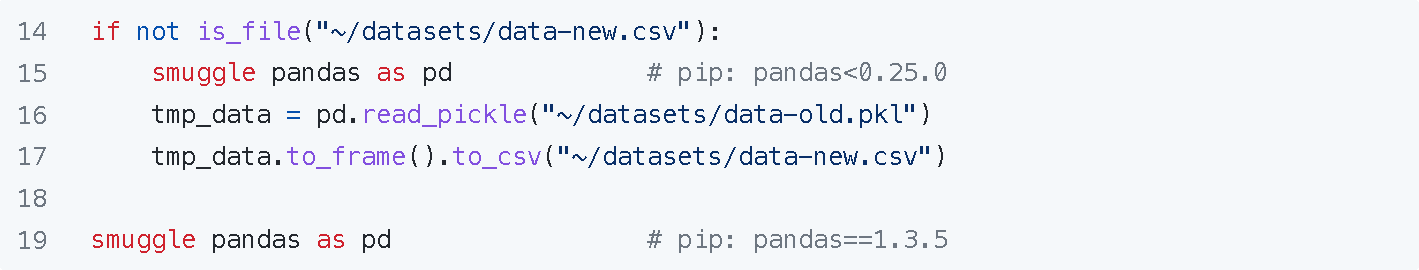
\includegraphics[width=0.9\textwidth]{figs/example4}
\end{center}

After re-enabling these two options (line 20), we next \texttt{smuggle}
specific versions of three plotting packages:
\texttt{Matplotlib}~\cite{Hunt07}, \texttt{seaborn}~\cite{Wask21}, and
\texttt{Quail}~\cite{HeusEtal17} (lines 22--24). Because the first two
are requirements of \texttt{UMAP}'s optional ``plot'' feature, they
will have already been installed by line 19, though possibly as
different versions than those specified in the onion comments on lines
22 and 23. If the installed and specified versions are the same, these
\texttt{smuggle} statements will function like standard \texttt{import}
statements to load the packages into the notebook namespace. If they
differ, Davos will download the requested versions in place
of the installed versions before doing so.
\begin{center}
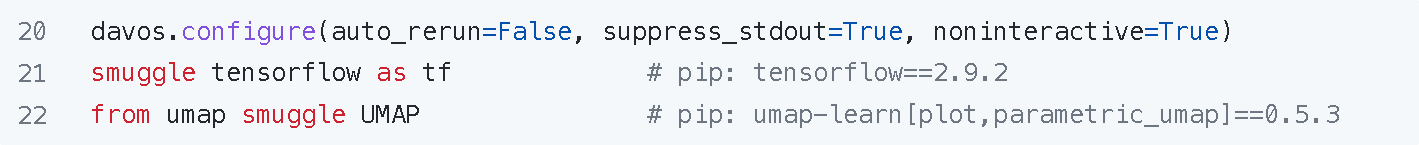
\includegraphics[width=0.9\textwidth]{figs/example5}
\end{center}
Line 24 uses an onion comment to specify that \texttt{Quail} should be
installed directly from a specific GitHub commit (\texttt{6c847a4}).
This ability to load packages directly from GitHub repositories can
enable developers to more easily use forked or modified versions of other
packages in their notebooks, even if those versions have not been
officially released.

In lines 26--29, we demonstrate another aspect of Davos's
functionality that supports more advanced installation scenarios.  The
\texttt{ipywidgets}~\cite{FredEtal15} package provides an API for
creating various JavaScript widgets with Python code, and the \texttt{widgetsnbextension} package provides
the machinery needed by the notebook frontend to display them.
\begin{center}
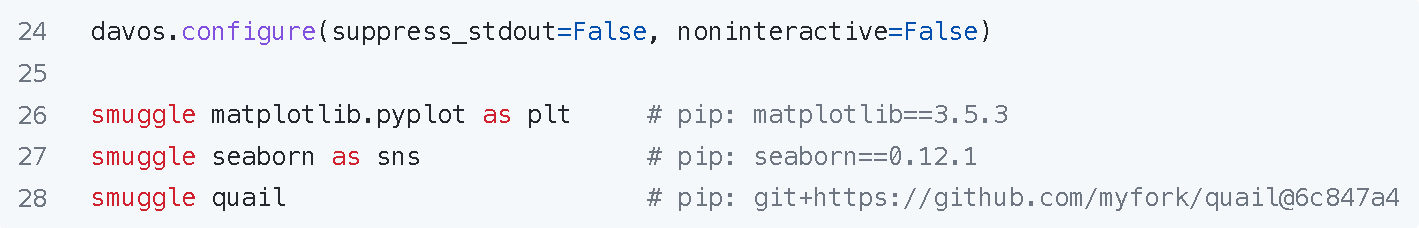
\includegraphics[width=0.9\textwidth]{figs/example6}
\end{center}
A complication is that \texttt{ipywidgets} must be installed in the
same environment as the IPython kernel, whereas
\texttt{widgetsnbextension} must be installed in the environment that
houses the Jupyter notebook server. In many basic setups, these two
environments are the same.  However, a common ``advanced'' approach
entails running the notebook server from a base environment, with
additional environments each providing their own separate,
interchangeable IPython kernels.  To accommodate this multi-environment
scenario, on lines 26 and 28, we use the \texttt{pip\_executable} option to control which environments each
package should be installed to.  Once these two packages are installed
and imported, line 31 smuggles \texttt{tqdm}~\cite{daCoEtal22}, which
display progress bars to provide status updates for running code. In
Jupyter notebooks, the \texttt{tqdm.notebook} module can be imported
to enable more aesthetically pleasing progress bars that are displayed via
\texttt{ipywidgets}, if that package is installed and
importable. Therefore, to take advantage of this feature, it was
important to \texttt{smuggle} \texttt{tqdm} after ensuring the
\texttt{ipywidgets} package was available.

Next, we load in the reformatted dataset (line 33) and pre-trained
model (line 35) that we wish to use in our analysis.  In our
hypothetical example, we can suppose that the model was provided as a
\texttt{scikit-learn} \texttt{Pipeline} object that passes data
through two pretrained models in succession.  First, a trained \texttt{CountVectorizer}
instance converts text data to an array of word counts.  Second, the
word counts are passed to a topic model~\cite{BleiEtal03} using a
pretrained \texttt{LatentDirichletAllocation} instance.
\begin{center}
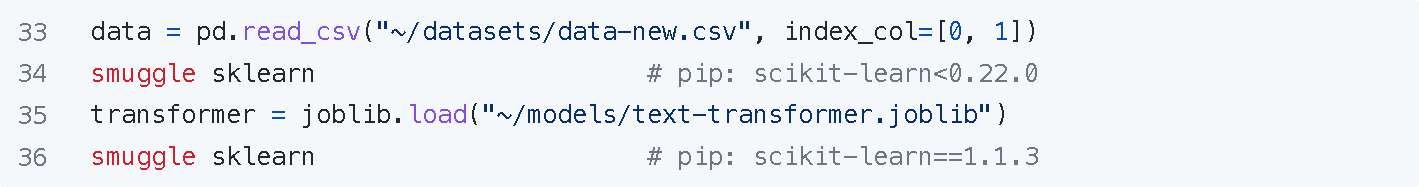
\includegraphics[width=0.9\textwidth]{figs/example7}
\end{center}
Let us suppose that the \texttt{Pipeline} object had been saved by its
original creator using the \texttt{joblib} package, as
\texttt{scikit-learn}'s documentation recommends.  Because
\texttt{joblib} uses the \texttt{pickle} protocol internally, the
ability to save and load pre-trained models is not guaranteed across
different \texttt{scikit-learn} versions.  For example, suppose that
the \texttt{Pipeline} object was created using \texttt{scikit-learn}
v0.21.3.  In that version of \texttt{scikit-learn}, the
\texttt{LatentDirichletAllocation} class was defined in
\texttt{sklearn.decomposition.online\_lda}.  However, in version
0.22.0, that module was renamed to \texttt{\_online\_lda}, and in
version 0.22.1, it was again renamed to \texttt{\_lda}.

In order to correctly load the model that includes the pre-trained
\texttt{LatentDirichlet\-Allocation} instance, in line 34, we first
\texttt{smuggle} a version of \texttt{scikit-learn} prior to v0.22.0 (i.e.,
before the first time the relevant module's name was changed).  Once
the model is loaded and reconstructed in memory from a compatible
package version (line 35), we upgrade to a newer version of
\texttt{scikit-learn} in line 36.  Taken together, the code in
Figure~\ref{fig:illustrative-example} shows how Davos can
enable users to load in data and models that are incompatible with
newer versions of \texttt{pandas} and \texttt{scikit-learn}, but still
\textit{analyze} and manipulate the data and model output using the
latest approaches and implementations.


\section{Impact}

Like virtual environments, containers, and virtual machines, the
Davos package (when used in conjunction with Jupyter
notebooks) provides a light\-weight mechanism for sharing code and
ensuring reproducibility across users and computing environments
(Fig.~\ref{fig:code-sharing}). Further, Davos enables users
to fully specify (and install, as needed) any project dependencies
within the same notebook. This provides a system whereby executable
code (along with text and media) \textit{and} code for setting up and
configuring the project dependencies, may be combined within a single
notebook file.

Although existing notebooks \textit{can} incorporate system calls that install
project requirements, handling project requirements in the general case is
non-trivial (e.g., see Fig.~\ref{fig:flow-chart}). Further, Davos
incorporates its own virtual environment system that isolates
notebook-installed packages from the runtime environment
(Sec.~\ref{subsec:projects}). In many setups this feature can eliminate the
need to set up a separate virtual environment or container (e.g., in
conjunction with a \texttt{requirements.txt}, \texttt{project.toml}, or
\texttt{environment.yml} file specifying the project's dependencies).

We designed Davos for use in research applications. For
example, in many settings, Davos may be used as a drop-in
replacement for more-difficult-to-set-up virtual environments,
containers, and/or virtual machines. For researchers, this lowers
barriers to sharing code. By eliminating most of the setup costs of
reconstructing the original researchers' computing environment,
Davos also lowers barriers to entry for members of the
scientific community and the public who seek to run shared code.

Beyond research applications, Davos is also useful in
pedagogical settings. For example, in programming courses, instructors
and students may use the Davos package to ensure their
notebooks will run correctly on others' machines. When combined with
online notebook-based platforms like Google Colaboratory,
Davos provides a convenient way to manage dependencies within
a notebook, without requiring any software (beyond a web browser) to
be installed on the students' or instructors' systems. For the same
reasons, Davos also provides an elegant means of sharing
ready-to-run notebook-based demonstrations or tutorials that install
their dependencies automatically.

Since its initial release, Davos has found use in a variety of applications. In
addition to managing computing environments for multiple prior and ongoing
research studies~\citep{MannEtal23a, OwenMann23, ZimaEtal23}, Davos is being
used by both students and instructors in programming and methods courses such
as Storytelling with Data~\cite{Mann21a} (an open course on data science,
visualization, and communication), Laboratory in Psychological
Science~\cite{Mann22} (an open course on experimental and statistical methods
for psychology research), and the Methods in Neuroscience at Dartmouth (MIND)
Computational Summer School~\cite{MIND23} (a week-long intensive course on
computational neuroscience methods) to simplify distributing lessons
and submitting assignments, as well as in online demos such as
\texttt{abstract2paper}~\cite{Mann21b} (an example application of
GPT-Neo~\cite{GaoEtal20, BlacEtal21}) to share ready-to-run code that installs
dependencies automatically. The 2023 offering of Neuromatch
Academy~\cite{vanVEtal21} also included an ``experimental'' module that uses
Davos to manage dependencies related to a large language model-based
tutor~\cite{MannEtal23b}.

Our work also has several more subtle ``advanced'' use cases and potential
impacts. Whereas Python's built-in \texttt{import} statement is agnostic to
packages' version information, \texttt{smuggle} statements (when combined with
onion comments) are version-sensitive. And because onion comments are parsed at
runtime, required packages and their specified versions are installed in a
just-in-time manner. Thus, it is possible in most cases to \texttt{smuggle} a
specific package version or revision even if a different version has already
been loaded. This enables more complex uses that take advantage of multiple
versions of a package within a single interpreter session (e.g., see
Sec.~\ref{sec:illustrative-example} and Fig.~\ref{fig:illustrative-example}).
This could be useful in cases where specific features are added or removed from
a package across different versions, or in comparing the performance or
functionality of particular features across different versions of the same
package.

A second more subtle impact of our work is in providing a
proof-of-concept of how the ability to add new ``keyword-like''
operators to the Python language could be specifically useful to
researchers. With Davos, we accomplish this by leveraging
IPython notebooks' internal code parsing and execution machinery. We
note that, while other popular packages similarly use these mechanisms
to providing notebook-specific functionality (e.g.,
\cite{Hunt07,HeusEtal18}), this approach also has the potential to be
exploited for more nefarious purposes. For example, a malicious user
could design a Python package that, when imported, substantially
changes the notebook's functionality by adding new \textit{unexpected}
keyword-like objects (e.g., based around common typos). We also note
that this implementation approach means Davos's functionality
is currently restricted to IPython notebook environments. However,
there have been early-stage discussions of providing this sort of
syntactic customizability as a core feature of the Python language,
including a draft proposal~\cite{Shan20}. In addition to enabling
Davos to be extended for use outside of notebooks, this could
lead to exciting new tools that, like Davos, extend the
Python language in useful and more secure ways.

\subsection{Pitfalls and limitations}

While Davos enables developers to conveniently specify all project
dependencies, there are some edge cases and limitations that are worth
considering. First, reproducibility is not solely about dependency management.
In addition to ensuring that project dependencies are satisfied, the user
running a given notebook must also execute the code in the indicated order. For
example, the cells in a notebook may be manually run out of order. If different
cells in a Davos-enhanced notebook made use of different versions of the same
package, this could result in \textit{more} confusion or \textit{greater}
replication failure rates relative to standard Jupyter notebooks. Therefore an
important consideration when using Davos is that it is perhaps even more
important to execute notebook cells in order than would be the case in the
standard (non-Davos) setup. One approach to mitigating this risk for notebooks
that use several versions of the same library would be to include
\texttt{smuggle} statements in the same cell(s) where the library was called. A
second approach would be for developers who wish to use Davos to include notes
regarding which cells must be executed in sequence. This is already a common
practice for notebooks that include system calls to install required packages
and dependencies, and the same approach would work well for Davos-enhanced
notebooks as well.

A second limitation of Davos relates to how packages are installed and managed.
As of this writing, Davos can install packages using \texttt{pip}, but not
other standard Python package management systems such as \texttt{conda}.
Therefore packages that are not installable via \texttt{pip} are currently
unsupported by Davos. We anticipate adding support for other package management
systems, including \texttt{conda}, in a future release.

A third limitation of Davos is that it cannot be used to manage projects that
depend on non-Python software. For example, system software or libraries from
other languages (e.g., in a mixed Python and R notebook), cannot be
\texttt{smuggle}d by Davos. A notebook that utilizes or depends on non-Python
software would therefore need to use existing non-Davos approaches to managing
those requirements.

\textcolor{red}{\textbf{TODO: add note about default/fallback project for non-traditional notebook interfaces}}

\section{Conclusions}

The Davos package supports reproducible research by providing
a novel, lightweight system for sharing notebook-based code. But
perhaps the most exciting uses of the Davos package are those
that we have \textit{not} yet considered or imagined. We hope that the
research and scientific Python communities will find Davos to provide a convenient
means of managing project dependencies to facilitate code sharing and collaboration. We
also hope that some of the more advanced applications of our package
might lead to new insights or discoveries.


\section*{Author Contributions}

\textbf{Paxton C. Fitzpatrick}: Conceptualization, Methodology,
Software, Validation, Writing - Original Draft,
Visualization. \textbf{Jeremy R. Manning}: Conceptualization,
Resources, Validation, Writing - Review \& Editing, Visualization, Supervision,
Funding acquisition.

\section*{Funding}

Our work was supported in part by NSF grant number 2145172 to JRM.
The content is solely the responsibility of the authors and does not
necessarily represent the official views of our supporting
organizations.


\section*{Declaration of Competing Interest}

We wish to confirm that there are no known conflicts of interest
associated with this publication and there has been no significant
financial support for this work that could have influenced its
outcome.


\section*{Acknowledgements}

We acknowledge useful feedback and discussion from the students of
JRM's \textit{Storytelling with Data} course (Winter, 2022 offering)
who used preliminary versions of our package in several assignments,
and the students of the Methods in Neuroscience at Dartmouth (MIND)
Computational Summer School (2023 offering) who used our package
during several workshops and tutorials.


\bibliographystyle{elsarticle-num}
\bibliography{main}

\end{document}
